\documentclass{beamer}
\usepackage{amsmath}
\usepackage[english]{babel} %set language; note: after changing this, you need to delete all auxiliary files to recompile
\usepackage[utf8]{inputenc} %define file encoding; latin1 is the other often used option
\usepackage{csquotes} % provides context sensitive quotation facilities
\usepackage{graphicx} %allows for inserting figures
\usepackage{booktabs} % for table formatting without vertical lines
\usepackage{textcomp} % allow for example using the Euro sign with \texteuro
\usepackage{stackengine}
\usepackage{wasysym}
\usepackage{tikzsymbols}
\usepackage{textcomp}
% ELIMINAR COMANDOS DE NAVEGACION%%%%%%%%%%%
\setbeamertemplate{navigation symbols}

%\newcommand{\bubblethis}[2]{
 %       \tikz[remember picture,baseline]{\node[anchor=base,inner sep=0,outer sep=0]%
 %       (#1) {\underline{#1}};\node[overlay,cloud callout,callout relative pointer={(0.2cm,-0.7cm)},%
 %       aspect=2.5,fill=yellow!90] at ($(#1.north)+(-0.5cm,1.6cm)$) {#2};}%
 %   }%
%\tikzset{face/.style={shape=circle,minimum size=4ex,shading=radial,outer sep=0pt,
 %       inner color=white!50!yellow,outer color= yellow!70!orange}}

%% Some commands to make the code easier
\newcommand{\emoticon}[1][]{%
  \node[face,#1] (emoticon) {};
  %% The eyes are fixed.
  \draw[fill=white] (-1ex,0ex) ..controls (-0.5ex,0.2ex)and(0.5ex,0.2ex)..
        (1ex,0.0ex) ..controls ( 1.5ex,1.5ex)and( 0.2ex,1.7ex)..
        (0ex,0.4ex) ..controls (-0.2ex,1.7ex)and(-1.5ex,1.5ex)..
        (-1ex,0ex)--cycle;}
\newcommand{\pupils}{
  %% standard pupils
  \fill[shift={(0.5ex,0.5ex)},rotate=80] 
       (0,0) ellipse (0.3ex and 0.15ex);
  \fill[shift={(-0.5ex,0.5ex)},rotate=100] 
       (0,0) ellipse (0.3ex and 0.15ex);}

\newcommand{\emoticonname}[1]{
  \node[below=1ex of emoticon,font=\footnotesize,
        minimum width=4cm]{#1};}
\usepackage{scalerel}
\usetikzlibrary{positioning}
\usepackage{xcolor,amssymb}
\newcommand\dangersignb[1][2ex]{%
  \scaleto{\stackengine{0.3pt}{\scalebox{1.1}[.9]{%
  \color{red}$\blacktriangle$}}{\tiny\bfseries !}{O}{c}{F}{F}{L}}{#1}%
}
\newcommand\dangersignw[1][2ex]{%
  \scaleto{\stackengine{0.3pt}{\scalebox{1.1}[.9]{%
  \color{red}$\blacktriangle$}}{\color{white}\tiny\bfseries !}{O}{c}{F}{F}{L}}{#1}%
}
\usepackage{fontawesome} % Social Icons
\usepackage{epstopdf} % allow embedding eps-figures
\usepackage{tikz} % allows drawing figures
\usepackage{amsmath,amssymb,amsthm} %advanced math facilities
\usepackage{lmodern} %uses font that support italic and bold at the same time
\usepackage{hyperref}
\usepackage{tikz}
\hypersetup{
    colorlinks=true,
    linkcolor=blue,
    filecolor=magenta,      
    urlcolor=blue,
}
\usepackage{tcolorbox}
%add citation management using BibLaTeX
\usepackage[citestyle=authoryear-comp, %define style for citations
    bibstyle=authoryear-comp, %define style for bibliography
    maxbibnames=10, %maximum number of authors displayed in bibliography
    minbibnames=1, %minimum number of authors displayed in bibliography
    maxcitenames=3, %maximum number of authors displayed in citations before using et al.
    minnames=1, %maximum number of authors displayed in citations before using et al.
    datezeros=false, % do not print dates with leading zeros
    date=long, %use long formats for dates
    isbn=false,% show no ISBNs in bibliography (applies only if not a mandatory field)
    url=false,% show no urls in bibliography (applies only if not a mandatory field)
    doi=false, % show no dois in bibliography (applies only if not a mandatory field)
    eprint=false, %show no eprint-field in bibliography (applies only if not a mandatory field)
    backend=biber %use biber as the backend; backend=bibtex is less powerful, but easier to install
    ]{biblatex}
\addbibresource{../mybibfile.bib} %define bib-file located one folder higher


\usefonttheme[onlymath]{serif} %set math font to serif ones

\definecolor{beamerblue}{rgb}{0.2,0.2,0.7} %define beamerblue color for later use

%%% defines highlight command to set text blue
\newcommand{\highlight}[1]{{\color{blue}{#1}}}


%%%%%%% commands defining backup slides so that frame numbering is correct

\newcommand{\backupbegin}{
   \newcounter{framenumberappendix}
   \setcounter{framenumberappendix}{\value{framenumber}}
}
\newcommand{\backupend}{
   \addtocounter{framenumberappendix}{-\value{framenumber}}
   \addtocounter{framenumber}{\value{framenumberappendix}}
}

%%%% end of defining backup slides

%Specify figure caption, see also http://tex.stackexchange.com/questions/155738/caption-package-not-working-with-beamer
\setbeamertemplate{caption}{\insertcaption} %redefines caption to remove label "Figure".
%\setbeamerfont{caption}{size=\scriptsize,shape=\itshape,series=\bfseries} %sets figure  caption bold and italic and makes it smaller


\usetheme{Boadilla}

%set options of hyperref package
\hypersetup{
    bookmarksnumbered=true, %put section numbers in bookmarks
    naturalnames=true, %use LATEX-computed names for links
    citebordercolor={1 1 1}, %color of border around cites, here: white, i.e. invisible
    linkbordercolor={1 1 1}, %color of border around links, here: white, i.e. invisible
    colorlinks=true, %color links
    anchorcolor=black, %set color of anchors
    linkcolor=beamerblue, %set link color to beamer blue
    citecolor=blue, %set cite color to beamer blue
    pdfpagemode=UseThumbs, %set default mode of PDF display
    breaklinks=true, %break long links
    pdfstartpage=1 %start at first page
    }


% --------------------
% Overall information
% --------------------
\title[Economía I]{Economía I \vspace{4mm}
\\ Magistral 6: Dentro de la firma II}
\date{}
\author[Ertola Navajas y Fariña]{Ertola Navajas y Fariña}
\vspace{0.4cm}
\institute[]{Universidad de San Andrés} 



\begin{document}

\begin{frame}
\titlepage
\centering
\includegraphics[scale=0.2]{Slides Principios de Economia/Figures/logoUDESA.jpg} 
\end{frame}



\begin{frame}
\frametitle{Entonces... ¿Cómo decidimos cuanto producir?}
\begin{itemize}
    \item Por un momento, supongamos que el precio de la pizza es p
        \item ¿Me conviene producir una pizza adicional?     
    \begin{itemize}
        \item Si uno aumenta una unidad de producto, recibe p
        \item Pero al mismo tiempo sus costos se incrementan en Cmg
        \item Entonces, el beneficio extra que se recibe es p – CMg
        \end{itemize}
    \item La diferencia entre el precio p y el costo marginal CMg se denomina ganancia marginal
\end{itemize}
\end{frame}

\begin{frame}
\frametitle{Conclusiones con un P fijo}
\begin{itemize}
    \item ¿Me conviene producir una pizza adicional?
        \begin{itemize}
        \item Si el beneficio marginal es positivo entonces SÍ conviene producir una pizza adicional
        \item Pero si el beneficio marginal es negativo entonces NO conviene producir una pizza adicional
        \end{itemize} 
    \item ¿Qué significa que el beneficio marginal sea igual 0?
\end{itemize}
\end{frame}

\begin{frame}
\frametitle{Vamos a ver que pasa con diferentes precios....}
\centering
\includegraphics[scale=0.6]{Slides Principios de Economia/Figures/Tema_06.20.jpg}
\end{frame}

\begin{frame}
\frametitle{La curva de oferta de la empresa}
%\centering
%\includegraphics[scale=0.6]{Slides Principios de Economia/Figures/Tema_06.28.jpg}

\begin{center}
\begin{figure}[H]
\renewcommand{\figurename}{Figure}
\begin{center}
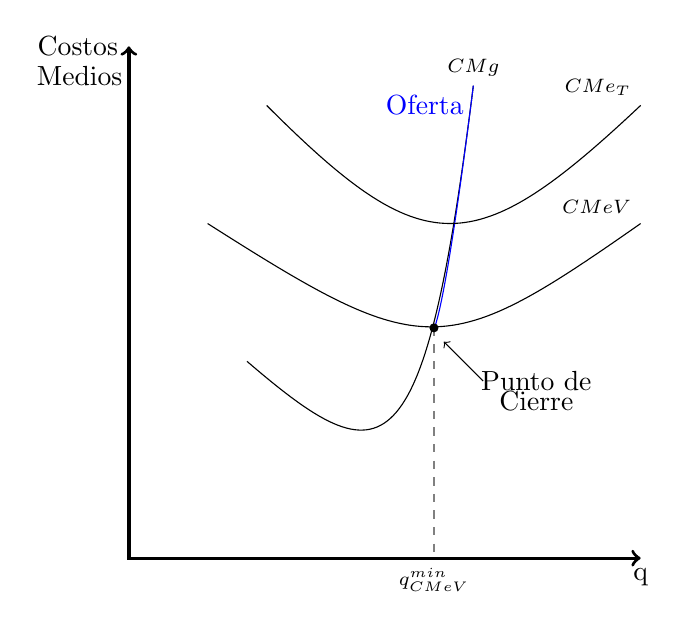
\begin{tikzpicture}[scale=0.5]
\draw[very thick,<->] (0,13) node[left]{Costos}--(0,0)--(13,0) node[below]{q};
\draw[thick,gray,dashed] (7.75,5.85)--(7.75,0);
\draw[thin] (3,5)..controls (6.5,2) and (7.5,2) .. (8.75,12) node[above] {\scriptsize $CMg$};
\draw[thin, blue] (7.75,5.8)..controls (7.75,5.9) and (8,6) .. (8.75,12) node[below left] {Oferta};
\draw[thin] (2,8.5)..controls (7.5,5) and (8,5) .. (13,8.5)node[above left] {\scriptsize $CMeV$};
 \draw[thin] (3.5,11.5)..controls (7.5,7.5) and (8.75,7.5) .. (13,11.5) node[above left] {\scriptsize $CMe_T$};
\node[below] at (7.75,0) {\scriptsize $q_{CMeV}^{min}$};
%\node[left] at (0,0) {\scriptsize $q_{CMeV}^{min}$};
\draw[fill] (7.75,5.85) circle [radius =0.1];
\draw[thin, <-] (8,5.5)--(9,4.5);
\node[] at (10.35,4.50) { Punto de};
\node[] at (10.35,4) {Cierre};
\node[below] at (-1.25,12.75) {Medios};
\end{tikzpicture}
\end{center}
\caption{\textbf{Punto de Cierre}}
\label{fig:C9.11}
\end{figure}
\end{center}
\end{frame}

\begin{frame}
\frametitle{La curva del mercado}

\begin{center}
\begin{figure}[H]
\renewcommand{\figurename}{Figure}
\begin{center}
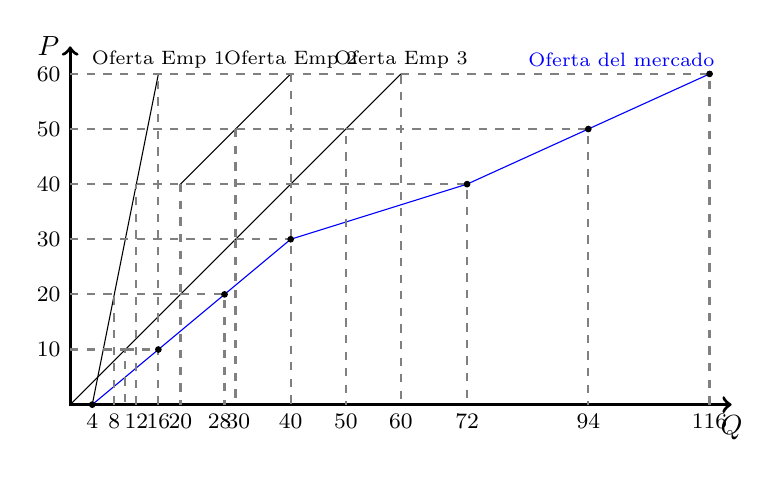
\begin{tikzpicture}[scale=0.35]
\draw[very thick,<->] (0,13) node[left]{$P$}--(0,0)--(24,0) node[below]{$Q$};
% Oferta Emp 3
\draw[thin](0,0)--(12,12);
% Oferta Emp 2
\draw[thin](4,8)--(8,12);
% Oferta Emp 1
\draw[thin](0.8,0)--(3.2,12);
% Oferta Mercado
\draw[thin, blue](0.8,0)--(8,6);
\draw[thin, blue](8,6)--(14.4,8);
\draw[thin, blue](14.4,8)--(23.2,12);

% Eje horizontal Emp 3 
\draw[thick,gray, dashed](0,2)--(2,2)--(2,0);
\draw[thick,gray, dashed](0,4)--(4,4)--(4,0);
\draw[thick,gray, dashed](0,6)--(6,6)--(6,0);
\draw[thick,gray, dashed](0,8)--(8,8)--(8,0);
\draw[thick,gray, dashed](0,10)--(10,10)--(10,0);
\draw[thick,gray, dashed](0,12)--(12,12)--(12,0);

% Eje horizontal Emp 1 
%\draw[thick,gray, dashed](2,6)--(2,2);
%\draw[thick,gray, dashed](1.2,0)--(1.2,2);
\draw[thick,gray, dashed](1.6,0)--(1.6,4);
\draw[thick,gray, dashed](2.4,0)--(2.4,8);
%\draw[thick,gray, dashed](2.8,0)--(2.8,10);
\draw[thick,gray, dashed](3.2,0)--(3.2,12);

% Eje horizontal Emp 2
\draw[thick,gray, dashed](4,8)--(4,4);
\draw[thick,gray, dashed](6,10)--(6,6);
\draw[thick,gray, dashed](8,12)--(8,8);

% Eje horizontal Oferta mercado 
\draw[thick,gray, dashed](2,2)--(3.2,2);
\draw[thick,gray, dashed](4,4)--(5.6,4)--(5.6,0);
\draw[thick,gray, dashed](6,6)--(8,6);
\draw[thick,gray, dashed](8,8)--(14.4,8)--(14.4,0);
\draw[thick,gray, dashed](10,10)--(18.8,10)--(18.8,0);
\draw[thick,gray, dashed](12,12)--(23.2,12)--(23.2,0);

% Eje vertical (todos comparten)
\node[left]at (0,4){\footnotesize 20};
\node[left]at (0,2){\footnotesize 10};
\node[left]at (0,6){\footnotesize 30};
\node[left]at (0,8){\footnotesize 40};
\node[left]at (0,10){\footnotesize 50};
\node[left]at (0,12){\footnotesize 60};
% Eje horizontal Emp 3 
%\node[below]at (2,0){\footnotesize 10};
\node[below]at (4,0){\footnotesize 20};
\node[below]at (6.1,0){\footnotesize 30};
\node[below]at (8,0){\footnotesize 40};
\node[below]at (10,0){\footnotesize 50};
\node[below]at (12,0){\footnotesize 60};
% Eje horizontal Emp 1
\node[below] at (0.8,0){\footnotesize 4};
%\node[below] at (1.2,0){\footnotesize 6};
\node[below] at (1.6,0){\footnotesize 8};
\node[below] at (2.4,0){\footnotesize 12};
%\node[below] at (2.8,0){\footnotesize 14};
\node[below] at (3.2,0){\footnotesize 16};

% Curva del oferta del mercado
\draw[fill] (0.8,0) circle [radius =0.1];
\draw[fill] (3.2,2) circle [radius =0.1];
\draw[fill] (5.6,4) circle [radius =0.1];
\draw[fill] (8,6) circle [radius =0.1];
\draw[fill] (14.4,8) circle [radius =0.1];
\draw[fill] (18.8,10) circle [radius =0.1];
\draw[fill] (23.2,12) circle [radius =0.1];
% Eje horizontal Curva de oferta
\node[below] at (23.2,0){\footnotesize 116};
\node[below] at (18.8,0){\footnotesize 94};
\node[below] at (14.4,0){\footnotesize 72};
\node[below] at (5.42,0){\footnotesize 28};

% Nombres 
\node[] at (3.2, 12.5) {\scriptsize Oferta Emp 1};
\node[] at (8, 12.5) {\scriptsize Oferta Emp 2};
\node[] at (12, 12.5) {\scriptsize Oferta Emp 3};
\node[, blue] at (20, 12.5) {\scriptsize Oferta del mercado};

\end{tikzpicture}
\end{center}
\caption{La curva de oferta del mercado}
\label{fig:C13.7}
\end{figure}
\end{center}
\end{frame}

\begin{frame}
\frametitle{En el largo plazo tenemos más flexibilidad}
\begin{itemize}
    \item Los costos de una empresa dependen de su escala y el tipo de tecnología de producción
    \item Empresas grandes pueden ser más rentables que las pequeñas debido diversas ventajas:
    \begin{itemize}
        \item Ventajas tecnológicas \\
        - Producción a gran escala permite mejorar la especialización y bajar los costos
        \item Ventajas de costos \\
        - Por ejemplo, empresas grandes, con mayor poder de negociación, pueden comprar recursos en términos más favorables
        \item Ventajas de demanda \\
        - Por ejemplo, efectos de red (valor de la producción aumenta con el número de usuarios)
    \end{itemize}
\end{itemize}
\end{frame}

\begin{frame}
\frametitle{Rendimientos a escala}
\begin{itemize}
    \item ¿Qué sucede con la producción cuando aumentamos la cantidad de insumos productivos en la misma proporción?\vspace{2mm}
    \begin{itemize}
        \item La producción aumenta pero... ¿cuánto aumenta?\vspace{4mm}
    \end{itemize}
    \item Si la producción aumenta más que proporcionalmente, entonces la función de producción exhibe rendimientos crecientes a escala (Economías de escala o costos decrecientes a escala)
\end{itemize}
\end{frame}

\begin{frame}
\frametitle{Rendimientos a escala}
\begin{itemize}
    \item Si la producción aumenta proporcionalmente, entonces la función de producción exhibe rendimientos constantes a escala (Costos constantes a escala)\vspace{4mm}
    \item Si la producción aumenta menos que proporcionalmente, entonces la función de producción exhibe rendimientos decrecientes a escala (Deseconomías de escala o costos crecientes a escala)
\end{itemize}
\end{frame}

\begin{frame}
\frametitle{Costos en el largo plazo}
\centering
\includegraphics[scale=0.6]{Slides Principios de Economia/Figures/Tema_06.24.jpg}
\end{frame}

\begin{frame}
\frametitle{Costos en el largo plazo}
\centering
\includegraphics[scale=0.6]{Slides Principios de Economia/Figures/Tema_06.25.jpg}
\end{frame}

\begin{frame}
\frametitle{Costos en el largo plazo}
\centering
\includegraphics[scale=0.6]{Slides Principios de Economia/Figures/Tema_06.26.jpg}
\end{frame}

\begin{frame}
\frametitle{Costos en el largo plazo}
\centering
\includegraphics[scale=0.6]{Slides Principios de Economia/Figures/Tema_06.25_costos4.jpg}
\end{frame}

\end{document}





